\section{MARCO TEÓRICO}

En este capítulo se describen los principales temas de interés para comprender de mejor manera el proyecto mediante fundamentos teóricos. Realizando una descripción de las tecnologías utilizadas para el desarrollo de la investigación. Es necesario comprender temas relacionados con los tipos de aplicaciones, dispositivos móviles, tecnologías de comunicación, tarjetas y componentes electrónicos, actuadores y sensores del vehículo, además de los diferentes aportes tecnológicos de la actualidad relacionados con la mejora continua del vehículo.


\subsection{TIPOS DE APLICACIONES}



\paragraph{Aplicaciones Web:}

(\cite{MT-11}) Son aquellas desarrolladas bajo lenguajes de desarrollo principalmente con tecnología Web entre los que destacan HTML, CSS y JavaScript. Hoy en día el trabajar con un \textit{framework} para el desarrollo eficientiza los procesos y permite la escalabilidad de la aplicación. Se podría decir que este tipo de aplicaciones son muy usadas para brindar accesibilidad a la información desde cualquier dispositivo móvil sin importar el sistema operativo, ya que solamente se necesita contar con un navegador para acceder a esta debido a que se encuentran alojadas en un servidor que mediante un nombre de dominio asociado o la dirección pública se pueden acceder. Algunas de las ventajas y desventajas de estas son: \\



Ventajas
\begin{itemize}
\item  Pueden ser utilizadas desde cualquier dispositivo móvil sin importar el sistema operativo.
\item  Puede que requiera un coste para su desarrollo, peor este puede ser mínimo en comparación con las nativas.
\item  No requieren de ninguna aprobación para su publicación.
\end{itemize}
Desventajas
\begin{itemize}
\item  No pueden ser publicadas en plataformas para su distribución.
\item  No utilizan los recursos del sistema ni del dispositivo de manera óptima.
\end{itemize}


\paragraph{Aplicaciones Móviles:}

una aplicación móvil (\cite{MT-11}), es una aplicación informática desarrollada para ser ejecutada a través de un dispositivo móvil inteligente, tablet o cualquier otro dispositivo que cuente con un sistema operativo. Estas se encuentran en tiendas en línea, por medio de las cuales son accedidas por el público que desee usarlas.\\

Dentro de estas plataformas de distribución de las aplicaciones móviles, se podrá encontrar de dos tipos, gratis y de paga. Las aplicaciones móviles pueden ser nativas que son aquellas desarrolladas bajo un lenguaje y entorno de desarrollo específico, lo cual permite, que su funcionamiento sea muy fluido y estable para el sistema operativo que fue creada. Pero también es importante recordar, que todo en esta vida tiene su ventajas y desventajas, y que las aplicaciones nativas no son la excepciona. Las ventajas y desventajas de estas son:\\

Ventajas
\begin{itemize}
\item  Utilización de los recursos tantos del sistema como del hardware.
\item  Permite ser publicada en tiendas para su distribución.
\item  En su mayoría, no necesitan estar conectadas a Internet para su funcionamiento.
\end{itemize}

Desventajas
\begin{itemize}
\item  Solo pueden ser utilizadas por un dispositivo que cuente con el sistema para el cual fue desarrollada.
\item  Requiere de un costo para distribuirla en una tienda, y dependiendo el sistema, para el uso del entorno de desarrollo.
\item  Necesitan aprobación para ser publicadas en la plataforma.
\end{itemize}

\paragraph{Aplicaciones Híbridas:}

Las aplicaciones híbridas (\cite{MT-11}), como su nombre lo indica tienen un poco de cada tipo de las aplicaciones ya nombradas. Este tipo de aplicaciones se desarrollan utilizando lenguajes de desarrollo web y un \textit{framework} dedicado para la creación de aplicaciones híbridas, como por ejemplo \textit{phonegap}, \textit{titanium}, \textit{appacelerator}, \textit{Steroids}, entre otros. La facilidad que brinda este tipo de desarrollo es que no hay un entorno específico el cual hay que utilizar para su desarrollo y la mayoría de olas herramientas son de uso gratuito, también pudiendo integrarlo con las herramientas de aplicaciones nativas. Las ventajas y desventajas de este tipo de desarrollo de aplicaciones son:\\

Ventajas
\begin{itemize}
\item  Uso de los recursos del dispositivo y del sistema operativo
\item  El costo de desarrollo puede ser menor que el de una nativa
\item  Son multiplataforma
\item  Permite distribución a través de las tiendas de su respectiva plataforma.
\end{itemize}
Desventaja
\begin{itemize}
\item  La documentación puede ser un poco escasa y desordenada.
\item  No utilizan todos los gráficos nativos del dispositivo
\end{itemize}


\subsection{DISPOSITIVOS MÓVILES}


Tradicionalmente la tecnología móvil se ha relacionado con la telefonía móvil (\cite{MT-12}). Actualmente existen múltiples dispositivos que ofrecen la posibilidad de acceder a internet, ya sean teléfonos móviles, \textit{Smartphone}, ordenadores portátiles, PDA, tabletas, consolas de videojuegos portátiles, entre otros. Estos dispositivos evolucionan con gran rapidez para adaptarse a las necesidades de los usuarios y también del mercado y, así, aparecen todos los años nuevos dispositivos móviles o nuevas versiones de dispositivos ya existentes, no necesariamente de telefonía. El abaratamiento de los dispositivos, la reducción del tamaño de los mismos y el aumento de prestaciones favorecen la expansión del uso de los dispositivos móviles.  Existen diferentes sistemas operativos que operan en los dispositivos móviles desde los más simples hasta los más usados como es el caso de Android  y sus versiones.

\paragraph{Android:}
Es un sistema operativo desarrollado para dispositivos móviles como teléfonos inteligentes, tabletas, \textit{Smart TV}, entre otros. En la actualidad la \textit{Open Handset Alliance} la cual es liderada por Google\textregistered  ha desarrollado el sistema Android el mismo que se basó en una versión de \textit{Linux}. La empresa de Google ha proporcionado todas las herramientas para la creación de nuevas aplicaciones para los dispositivos móviles con sistema operativo Android, además de incluir un emulador de teléfono Android. A este conjunto de herramientas lo denominaron Android SDK utilizando la licencia de software libre. \\ 

El Android SDK trabaja conjuntamente con el software Android Studio, que es un potente entorno de desarrollo, libre y gratuito. El lenguaje de programación que utiliza Android Studio para el desarrollo de aplicaciones móviles es Java, por medio de sus líneas de programación se da la realización de las aplicaciones para los celulares con sistema operativo Android.\\

El futuro apunta a conexión inalámbrica y la tecnología Bluetooth es una de las que encabeza en el mundo de la tecnología donde el enlace de datos debe ser robusto, confiable y seguro. En la actualidad tenemos la facilidad de obtener modelos económicos en el mercado que se encuentran distribuidos por todo el mundo además de su sencillo uso para distintas aplicaciones desarrolladas para sistemas operativos Android.\\


\subsection{TECNOLOGÍAS DE COMUNICACIÓN}

\paragraph{WI-FI:}
son las siglas de Wireless Fidelity y comprende una gran cantidad de estándares para redes de comunicación inalámbrica basados en las especificaciones IEEE 802.11. En sus inicios Wi-Fi fue pensado para conectar redes locales inalámbricas; sin embargo, actualmente se utiliza para el acceso a Internet (\cite{MT-06}).\\ 

En Wi-Fi un punto de acceso inalámbrico transmite y recibe datos a través de ondas de radio y los equipos remotos, que cuentan con un transceptor (transmisor-receptor) en una tarjeta de acceso, se comunican con él como se muestra en la Figura \ref{Mcinco} (\cite{MT-07}).\\  

El punto de acceso inalámbrico se conecta a un MODEM que se comunica de manera cableada con el núcleo de la red. Por cuestiones de seguridad, mediante un esquema llamado WEP (Wired Equivalent Privacy) los datos reciben un tratamiento criptográfico con códigos de 128 bits y solo los usuarios con contraseña pueden acceder a la red (\cite{MT-08}). Hoy en día, se utiliza un esquema más robusto llamado WPA: Wi-Fi Protected Access.

%
\begin{figure}[H]
%\vspace{0.2cm}
\centering
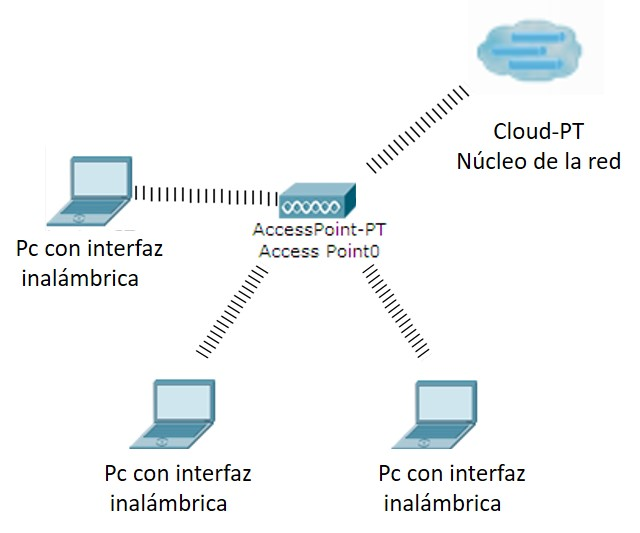
\includegraphics[width=0.5\textwidth]{marco/fig5.jpg}
\caption{Diagrama de una red Wi-Fi. }
\label{Mcinco}
\end{figure}
%

Wi-Fi es una tecnología de área local que alcanza tasas de transmisión de hasta 54 kbps en un canal de 20 MHz en la banda de 2.4 GHz (banda no licenciada) y opera con modulaciones por desplazamiento de fase, la cual es una forma de modulación angular que consiste en hacer variar la fase de la portadora entre un número de valores discretos (\cite{MT-09}). Es una plataforma bastante escalable y de fácil instalación. Sin embargo, no garantiza calidad de servicio (QoS del inglés \textit{Quality of Service} ) ni brinda mayor seguridad a la información que se transmite (\cite{MT-10}).



\paragraph{Bluetooth:}

En 1994, la compañía global de telecomunicaciones Ericsson Mobile Communications investigó la viabilidad de una interfaz de radio de baja potencia y ajo coste entre dispositivos móviles y sus accesorios, llegando a la conclusión de que dicho tipo de conexión debería ser un enlace de radio de corto alcance.\\

Esta investigación atrajo la atención de otras grandes compañías como IBM, Intel, Nokia y Toshiba, creando el SIG Bluetooth, consorcio inalámbrico que creció exponencialmente tras pocos años.\\

El nombre fue dado con motivo de honrar a un rey vikingo danés del sigo X. Haral Bluetooth, el cuál reinó desde el año 940 hasta el 985 y al que le atribuye la unificación del mencionado país y la adopción del cristianismo.\\
La relación entre el nombre y la tecnología Bluetooth es que lo que se pretende con ésta última es la unificación y armonía para permitir a diferentes dispositivos que se comuniquen a través de un estándar aceptado para la comunicación inalámbrica (\cite{MT-05}). \\

El conjunto de especificaciones Bluetooth desarrolladas por Ericsson y otras compañías responde a las necesidades de conectividad inalámbrica de corto alcance para redes ad hoc. Una red ad hoc es un tipo de red inalámbrica descentralizada, es decir, no depende de una infraestructura pre-existente. El protocolo de banda base de Bluetooth es una combinación de conmutación de circuitos y de paquetes, haciéndola idónea para transmitir tanto voz como para datos. \\

La tecnología Bluetooth se implementa en transceptores de corto alcance, de pequeño tamaño y bajo coste en dispositivos móviles, integrada de forma directa o mediante dispositivos adaptadores. La tecnología inalámbrica utiliza la banda de radio ISM mundialmente disponible de 2.4 GHz y no requiere licencia. Éstas bandas incluyen los rangos de frecuencia entre 902-928 MHz y 2.4-2.484 GHz que no requieren licencia de operador otorgada por las autoridades reguladoras de telecomunicaciones (\cite{MT-05}).\\

Los módulos de desarrollo bluetooth es un perfecto aliado para eliminar los cables en los proyectos o para conectarse a ordenadores y/o teléfonos móviles.\\

Tiene un alcance de hasta 100 metros seccionado por rangos de 10 metros, posee antena integrada, son compatibles con el resto de versiones Bluetooth, permite velocidades de transferencia de hasta 921 Kbps, y se puede conectar de forma sencilla mediante la UART(RX/TX) de cualquier micro controlador, desde donde se puede controlarlo haciendo uso de sencillos comandos AT.\\

Puede ser alimentado tanto a 5 Volts como a 3.3 Volts, y para ello dispone de un puente (jumper) de selección de la tensión de alimentación.\\

Para establecer una comunicación entre los dispositivos móviles se sigue un procedimiento para poder garantizar un cierto grado de seguridad entre los dispositivos conectados:
\begin{itemize}
\item modo pasivo,
\item solicitud, 
\item paginación,
\item descubrimiento del servicio del punto de acceso,
\item creación de un canal con el punto de acceso,
\item emparejamiento mediante el PIN(Seguridad),
\item utilización de la red.
\end{itemize}

En el modo pasivo el funcionamiento del dispositivo es normal, en la fase de Solicitud, la comunicación comienza durante la cual el principal envía una solicitud a los dispositivos que se encuentran dentro del rango, denominados los puntos de acceso, en la fase paginación el dispositivo principal elige una dirección o un punto de acceso que consta de una sincronización de su reloj y frecuencia, luego sigue la fase de descubrimiento de servicio, se establece un enlace con el punto de acceso mediante un protocolo denominado SDP (del inglés \textit{Service Discovery Protocol}), Cuando esta fase de descubrimiento de servicio finaliza, el dispositivo principal o maestro ya está listo para crear un calan de comunicación.\\

Un mecanismo de seguridad llamado emparejamiento, restringe el acceso a otros dispositivos, soló se aceptan dispositivos autorizados para brindar a la piconet cierto grado de proyección.\\

El emparejamiento se realiza mediante una clave de acceso conocida como PIN que es un Número de identificación Personal. Para esto se envía una solicitud al dispositivo de emparejamiento al dispositivo principal o maestro de tal manera que se deberá conocer la clave de acceso para llevar a cabo dicha conexión. \\
 





\paragraph{GSM}

 El Sistema Global para las comunicaciones móviles  (\cite{UPS-03}) es un sistema estándar, completamente definido para generar una comunicación entre teléfonos móviles que incorporan tecnología digital. Por ser digital cualquier usuario de GSM puede conectarse a través de su teléfono con su computadora además de poder enviar y recibir mensajes por email, faxes, navegar por internet, acceso seguro a la red informática de una compañía, así como utilizar otras funciones digitales de transmisión de datos incluyendo el servicio de mensajería cortos o mensajes de texto.\\

GSM se considera, por su velocidad de transmisión y otras características, un estándar actual de cuarta generación (4G). Una de las características principales del estándar GS es en Módulo de Identidad del Suscriptor (SIM por sus siglas en inglés). \\

La tarjeta SIM es una tarjeta inteligente desmontable que contiene la información de suscripción del usuario, parámetros de red y directorio telefónico. Esto permite al usuario mantener su información después de cambiar su teléfono. Paralelamente, el usuario también puede cambiar de operador de telefonía, manteniendo el mismo equipo, simplemente cambiando la tarjeta SIM.\\

Debido a que los mensajes SMS son recibidos prácticamente de inmediato por el destinatario y son un medio de comunicación muy personal, muchos ya los están utilizando como uno de los mejores medios para comunicación ante la sociedad.\\

\subsection{TARJETAS Y COMPONENTES ELECTRÓNICOS}

\paragraph{Arduino}

Antes de que aparecieran plataformas de hardware libre como Arduino, la creación de prototipos de sistemas \textit{software-hardware} era complejo y caro. Por ello, muchas universidades y centros de investigación empezaron a desarrollar alternativas más baratas y sencillas a finales del siglo XX. Pero estas soluciones no eran generales y su popularidad fuera de su institución era pequeña. Hasta que en 2005 nació Arduino en el instituto IVREA de Italia, como un proyecto para estudiantes dirigido por Massimo Banzi, que aplicaba los conceptos de \textit{hardware} y \textit{software} libres, lo que supuso un cambio importante (\cite{MT-01}).\\ 

El concepto de \textit{hardware} libre de Arduino hace referencia a un diseño de un sistema electrónico basado en microprocesador que está disponible de forma gratuita, para su uso o modificación. Además, el \textit{software} usado para programar el sistema es libre y de acceso gratuito, y fácil de obtener, poner en marcha y usar (\cite{MT-02}). \\

Todo esto ha hecho que los dispositivos de la plataforma Arduino (ver Figura \ref{Mtres}) se hayan popularizado y extendido enormemente, y sea posible encontrar soluciones disponibles de forma abierta, para prácticamente todo tipo de proyectos. Todos los dispositivos Arduino se programan fácilmente con el mismo entorno de desarrollo, mediante lenguaje C/C++, pudiéndose crear desde programas simples de un solo archivo basados en procedimientos, hasta programas complejos de múltiples archivos y orientados a objetos. También es fácil encontrar documentación en internet sobre cualquier aspecto de la plataforma Arduino, y hay gran cantidad de libros de texto para usuarios con distintos niveles de conocimientos (\cite{MT-03}). \\


%
\begin{figure}[H]
%\vspace{0.2cm}
\centering
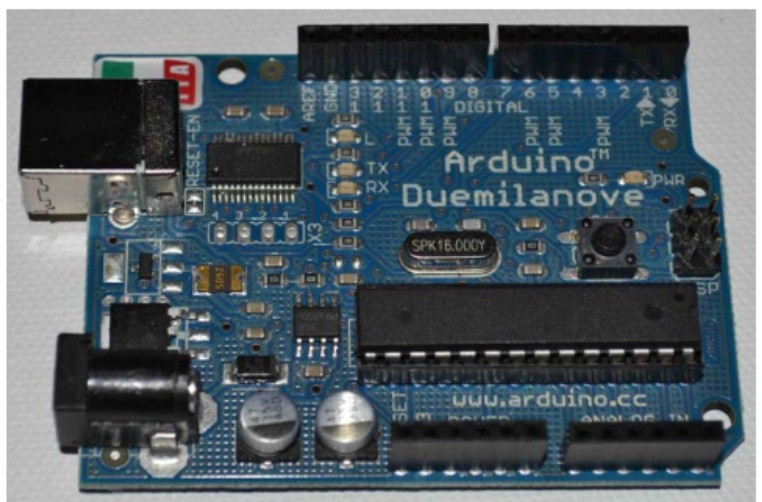
\includegraphics[width=0.5\textwidth]{marco/fig3.jpg}
\caption{Tarjeta Arduino \cite{MT-03}. }
\label{Mtres}
\end{figure}
%



\paragraph{Raspberry Pi}

La Raspberry Pi (ver Figura \ref{Mcuatro}) se comenzó a comercializar en agosto de 2011 con el objetivo de ser utilizada para incentivar el conocimiento en el uso de la electrónica y la programación en edades tempranas (\cite{MT-04}). Desde esa fecha ha transitado por 4 modelos, aumentando cada vez más su capacidad de procesamiento y prestaciones. Un modelo muy comercial es el B+, que cuenta con un procesador ARM a 700 MHz, 512 MB de memoria SDRAM (Synchronous Dynamic Random-Access Memory, en español, Memoria de Acceso Sincrónico, Dinámico y Aleatorio), salidas de video compuesto y HDMI (High-Definition Multimedia Interface, en español, Interface Multimedia de Alta Definición) hasta 1080p. Su almacenamiento es mediante tarjetas MicroSD; además posee un bajo consumo de energía llegando solamente a los 3.5 W. Además, cuenta con 40 pines de Entrada Salida de Propósito General (GPIO, del inglés \textit{General Purpose Input Output}) y el sistema operativo más usado para su operación es el Raspbian, una variante de Debían diseñada especialmente para ella.

%
\begin{figure}[H]
%\vspace{0.2cm}
\centering
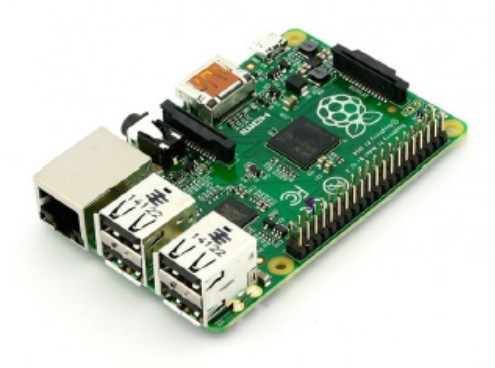
\includegraphics[width=0.5\textwidth]{marco/fig4.jpg}
\caption{Tarjeta Raspberry Pi \cite{UPS-08}. }
\label{Mcuatro}
\end{figure}
%

\paragraph{Relevador}
Un relevador es un interruptor accionado por un electroimán, un electroimán está formado por una barra de hierro dulce, llamada núcleo, rodeada por una bobina de hilo de cobre tal como se muestra en la Figura \ref{Muno}, al pasar una corriente eléctrica por la bobina el núcleo de hierro se magnetiza por efecto del campo magnético producido por la bobina, convirtiéndose en un imán tanto más potente cuanto mayor sea la intensidad de la corriente y el número de vueltas de la bobina. Al abrir de nuevo el interruptor y dejar de pasar corriente por la bobina, desaparece el campo magnético y el núcleo deja de ser un imán.

%
\begin{figure}[H]
%\vspace{0.2cm}
\centering
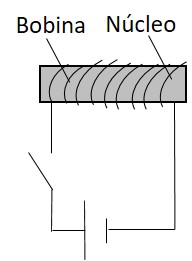
\includegraphics[width=0.4\textwidth]{marco/fig1.jpg}
\caption{Electróiman. }
\label{Muno}
\end{figure}
%

El relevador más sencillo está formado por un electroimán como el descrito anteriormente y un interruptor de contactos tal cual se muestra en la Figura \ref{Mdos}. Al pasar una pequeña corriente por la bobina, el núcleo se imanta y atrae al inducido por uno de sus extremos, empujándolo por el otro a uno de los contactos hasta que se juntan, permitiendo el paso de la corriente a través de ellos.

%
\begin{figure}[H]
%\vspace{0.2cm}
\centering
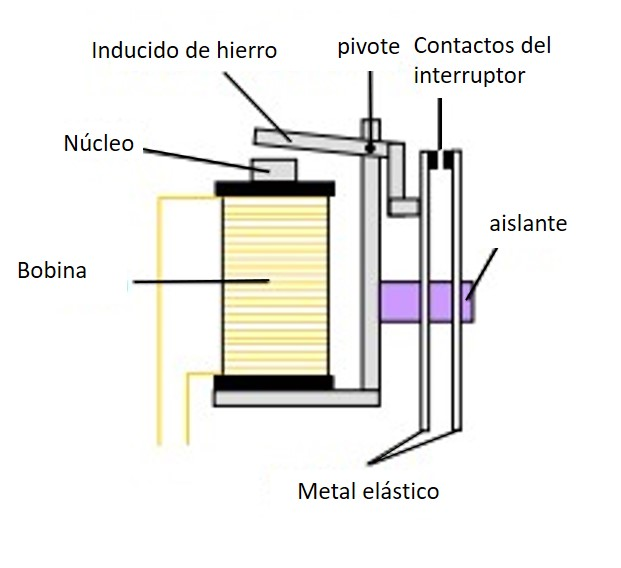
\includegraphics[width=0.5\textwidth]{marco/fig2.jpg}
\caption{Estructura del relevador. }
\label{Mdos}
\end{figure}
%

\subsection{SISTEMAS DEL VEHÍCULO}
Los sistemas principales que conforman un vehículo son el Sistema de Tracción y el Sistema de Confort. Estos están monitoreados por sensores y actuadores que apoyan la detección de fallas, además de la visualización de la información que envía el vehículo al conductor.\\

Los vehículos se clasificarán para este documento en tres principales gamas; ``gama baja", ``gama media" y ``gama alta". La clasificación de la gama depende de la seguridad y tecnología que esta implementada, entre mayor tecnología y seguridad mayor será la gama.\\


\subsection{ÁREAS DE MEJORA CONTINUA DEL VEHÍCULO}

\paragraph{GPS}

El sistema de posicionamiento global (GPS) en sus inicios comenzó como un proyecto militar hoy en día está disponible para su uso civil, operativo desde 1995 utiliza conjuntamente una red de computadora y una constelación de veinticuatro satélites para determinar por triangulación la altitud, longitud y latitud de cualquier objeto en la superficie terrestre (\cite{MT-13}).\\

El GPS es un sistema que tiene como objetivo la determinación de las coordenadas espaciales de puntos respecto de un sistema de referencia mundial. Los puntos pueden estar ubicados en cualquier lugar del planeta, pueden permanecer estáticos o en movimiento y las observaciones pueden realizarse en cualquier momento del día (\cite{MT-13}).\\

El sistema se descompone en tres segmentos básicos según Eduardo, Aldo y Gustavo mencionan en (\cite{MT-14}):

\subparagraph{Segmento espacio o espacial}

Formado por 24 satélites GPS con una órbita de 26 560 Km. De radio y un periodo de 12 horas. Cabe mencionar que a estos satélites se les incorporo la señal de una perturbación denominada SA (Selective Availability) que no es otra cosa que la disminución intencional de la precisión del sistema, también se estableció una limitación al acceso del denominado código P. Estas características fueron impuestas a los usuarios civiles por cuestiones de interés militar.


\subparagraph{Segmento control}

Consta de cinco estaciones monitoras encargadas de mantener en órbita los satélites y supervisar su correcto funcionamiento, tres antenas terrestres que envían a los satélites las señales que deben transmitir y una estación experta de supervisión de todas las operaciones.\\

Las funciones principales del segmento de control, denominado internacionalmente con las siglas OCS (del inglés \textit{Operational Control Segment}) son: monitoreo y control permanente de los satélites con el objeto de determinar y predecir las órbitas y los relojes de a bordo, la sincronización de los relojes de los satélites con el tiempo GPS y la transmisión, a cada satélite, de la información procesada.\\

El segmento control está integrado por 10 estaciones las cuales se ubican en \textit{Colorado Springs} (EUA), Isla Ascensión (Atlántico Sur), Diego García (Indico), \textit{Kwajalein} (Pacifico Occidental), \textit{Hawái} (Pacifico Oriental), Quito (Ecuador), Buenos Aires (Argentina), Hermitage (Inglaterra), \textit{Bahrain} (Golfo Pacifico), \textit{Smithfield} (Australia) como se muestra en la Figura \ref{Mseis}.


%
\begin{figure}[H]
%\vspace{0.2cm}
\centering
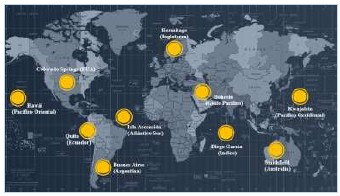
\includegraphics[width=0.5\textwidth]{marco/fig7.jpg}
\caption{Segmento control GPS.}
\label{Mseis}
\end{figure}
%


\subparagraph{Segmento usuario}
Está constituido por los instrumentos utilizados para la recepción y procesamiento de la señal emitida por los satélites, formado por las antenas y los receptores pasivos situados en tierra. La antena está conectada por cable al receptor o en otros casos forman una sola unidad.\\

Las coordenadas que se calculan corresponden al centro radioeléctrico de la antena. El receptor consta de un mínimo de 4 canales (generalmente 10 o 12) que permiten recibir y procesar simultáneamente la señal de cada satélite. Posee además un oscilador de cuarzo que permite generar la frecuencia de referencia para realizar la observación. \\

Un microprocesador interno con el \textit{software} correspondiente calcula las coordenadas de la antena y la velocidad y acimut si el aparato está en movimiento.\\

Las características que posee el sistema GPS son las siguientes:
\begin{itemize}
\item Compuesto por 24 satélites.
\item Los satélites se ubican en 6 órbitas planas prácticamente circulares, con inclinación de 55º respecto al plano del Ecuador y con una distribución aproximadamente uniforme; con 4 satélites en cada órbita.
\item Se encuentran aproximadamente a 20, 180 km de altura.
\item Tienen 12 h. de período de rotación (en tiempo sidéreo) u 11 h. 58 min. (en tiempo oficial).
\item También hay satélites en órbita que se encuentran desactivados y disponibles como reemplazo.
\item Con la constelación completa, se dispone, en cualquier punto y momento, entre 5 y 11 satélites observables, con geometría favorable.
\item El tiempo máximo de observación de un satélite es de hasta 4 horas 15 minutos.
\end{itemize}

\paragraph{Seguridad Vehícular}

La seguridad vehicular es el conjunto de elementos y sistemas ubicados en el automotor para que el usuario se encuentre protegido de todo daño o riesgo en caso de un accidente de tránsito. Estos dispositivos dotan a los vehículos de los más altos niveles de seguridad y de mejores condiciones para una conducción adecuada.

La principal misión de la seguridad vehicular es la de proteger la integridad física y psicológica del conductor y de los ocupantes, antes y en el momento que se provoque el accidente, por medio de la reducción de los riesgos y la limitación de las consecuencias del impacto.

El objetivo principal de este sistema es disminuir el riesgo de accidentes que se pueden producir durante el uso regular y habitual del vehículo, por lo cual los dispositivos y elementos que lo conforman deben garantizar que el conductor no sufra perturbaciones en la marcha del vehículo y además que se facilite la manipulación de los mandos que permiten que éste pueda funcionar.

De acuerdo a la funcionabilidad de los diferentes dispositivos y elementos que conforman este sistema, se puede clasificar (\cite{MT-15}):
\begin{itemize}
	\item Seguridad de marcha: Tiene como objetivo garantizar el correcto funcionamiento dinámico del vehículo en los mecanismos de dirección, frenos, suspensión y conjuntos de trasmisión de las ruedas.

	\item Sistema en la percepción de señales: Se determina por el buen estado y aplicación de los dispositivos de iluminación, dispositivos acústicos de advertencia y medidas de visión.

	\item Seguridad de servicio: Establece la facilidad que brinda el vehículo para poder manipular los mandos y controles durante la conducción de manera confortable
\end{itemize}
Por otra parte, el sistema de seguridad pasivo tiene la finalidad de disminuir las consecuencias posteriores a un accidente, para esto se debe tener en cuenta el comportamiento de la estructura del vehículo en el momento del impacto y luego del mismo, además de la utilización de mecanismos y elementos que detengan o disminuyan la evolución del accidente.\\
\begin{itemize}
	\item
Seguridad interior: Tiene como objetivo precautelar el estado de supervivencia de los ocupantes del vehículo cuando se provoca un accidente buscando reducir el impacto y facilitando la liberación de los accidentados.\\
\end{itemize}

Dentro de las medidas de protección se tiene el comportamiento de la deformación de la carrocería en el habitáculo, sistemas de sujeción, fijación de parabrisas, elementos de protección, etc.\\
\begin{itemize}
	\item
Seguridad exterior: Busca reducir las lesiones de las personas que al estar involucradas en el accidente no son ocupantes del vehículo, por lo que en este caso influye el comportamiento de la carrocería ante el impacto y la forma exterior que tiene la misma.\\
\end{itemize}
Dentro de las medidas de seguridad se debe considerar la disposición y aplicación de elementos como faros, limpiaparabrisas, manecillas, etc. (\cite{MT-15}).


\paragraph{Sistema de iluminación del vehículo}

El sistema de iluminación, clave en la seguridad activa de un vehículo, proporciona la cantidad adecuada de luz para la correcta conducción del automotor en diferentes situaciones adversas de visibilidad; a través de dispositivos lumínicos tales como luces incandescentes, leds, faros, neón, halógeno, ver Figura \ref{Mcinco2}, que en conjunto y en una distribución adecuada sirven de localización, información y advertencia de acciones ejecutadas por el conductor.\\

Normas internacionales de calor de luz ayudan a interpretar de mejor manera la funcionalidad de cada dispositivo lumínico; faros traseros de color rojo, laterales o direccionales color ámbar y faros delanteros color amarillo o blanco.

De acuerdo a la ubicación de los dispositivos lumínicos, podemos dividir el sistema de iluminación en tres grupos:
\begin{itemize}
	\item
	Faros y luces auxiliares de iluminación delantera.
    	\item
	Faros frontales, laterales y traseros de señalización.
    	\item
	Luz interior y otros dispositivos lumínicos.
\end{itemize}
%
\begin{figure}[H]
%\vspace{0.2cm}
\centering
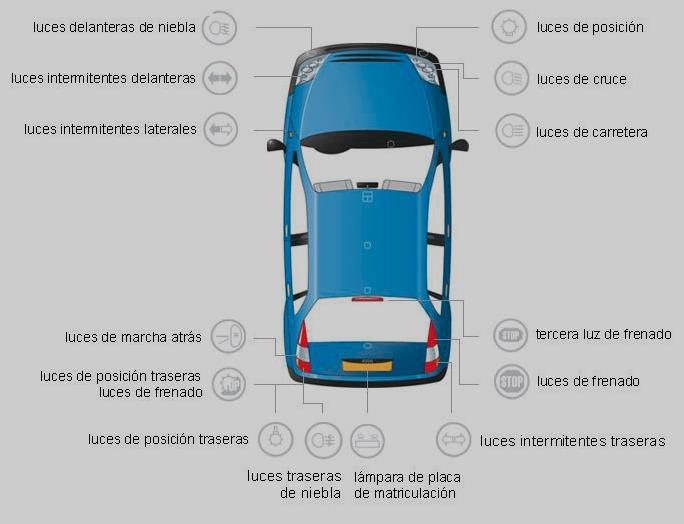
\includegraphics[width=0.5\textwidth]{marco/fig6.jpg}
\caption{Sistema de iluminación general de un vehículo.}
\label{Mcinco2}
\end{figure}
%

\paragraph{Sistema de alarma de seguridad}

Un sistema de alarma es un elemento de seguridad activa que permite advertir al conductor de situaciones anormales en el vehículo, y ejecutar una acción rápida de acuerdo al problema presente. 

En la actualidad la mayoría de las alarmas modernas están constituidas por distintos tipos de sensores, interruptores, sirenas, receptor de radio para control inalámbrico, batería auxiliar de alimentación del sistema de alarma y una unidad central de monitoreo.

De acuerdo a la tecnología utilizada y al propósito del sistema de alarma, se puede distinguir un sistema antirrobo y un sistema de seguridad centralizado.

\textbf{Sistema Antirrobo:}
Es la forma básica de un sistema de alarma, formada por una centralita que gestionara el activar de todos los interruptores, sensores, dispositivos sonoros del vehículo; además de un mecanismo traba volante y corta corriente.

\textbf{Sistema de seguridad centralizado:}
Cumple la función principal de todo sistema de alarma convencional y adicionalmente bloquea el vehículo en su totalidad, impidiendo apertura desde el interior y exterior. Utiliza tecnología más sofisticada con una unidad central que puede desconectar si es necesario el computador o cerebro del automotor. 

Distintas tecnologías aplicadas como GPS utilizada para la localización exacta a través de un centro de operaciones; una alarma silenciosa que lleva un registro celular que informa vía SMS de la situación actual el vehículo; un sistema Keyless para el encendido electrónico sin la necesidad de utilizar llaves. 

Vehículos de nueva generación incorporan sistemas biométricos en sus unidades aprovechando las características únicas que estos ofrecen como son lectores de retina, huella dactilar, reconocimiento facial, reconocimiento de voz
 \cite{MT-16}.

